\section{Synteny}

\subsection{Introduction}

\subsection{Methods}

\subsubsection{Data sets}


The \emph{Ae. aegypti}, \emph{An. gambiae}, \emph{L. longipalpis}, and \emph{P. papatasi} \textcolor{red}{TODO VERSIONS} peptide translations were downloaded from Vectorbase \textcolor{red}{TODO CITE}, while the \emph{D. melanogaster} and \emph{D. simulans} peptide translations were downloaded from Flybase \textcolor{red}{TODO CITE}.

\textcolor{red}{table of versions}


\subsubsection{Calculation of Scaffold Gene CDF}
The gene counts of each genome's scaffolds were normalized by dividing the gene counts by the number of genes in that organism's genome. For each genome, the scaffolds were sorted by their gene counts largest to smallest.  A cumulative sum was computed over the normalized gene counts.   The normalized cumulative size of each scaffold was plotted. For genomes which had few scaffolds than the largest genome, the plots were extended to the largest number of scaffolds among all of the organisms with points of value 1.


\subsubsection{Generation of Dot Plots for Macrosynteny}
The identifiers, scaffolds, locations, and sense in the FASTA headers were extacted for each peptide sequence (Figure~\ref{fig:synteny-workflow}).  The protein IDs were cross-referenced with OrthoDB to group the proteins into ortholog groups.  Sequences without ortholog information or no orthologs in the other genomes and ortholog groups with many-to-many and one-to-many relationships were discarded.  The proteins were sorted along each scaffold by their starting coordinates, while scaffolds were ordered arbitrarily.  Scatter plots were generated by drawing dots at the positions of orthologous proteins.

\begin{figure}[H]
  \centering
  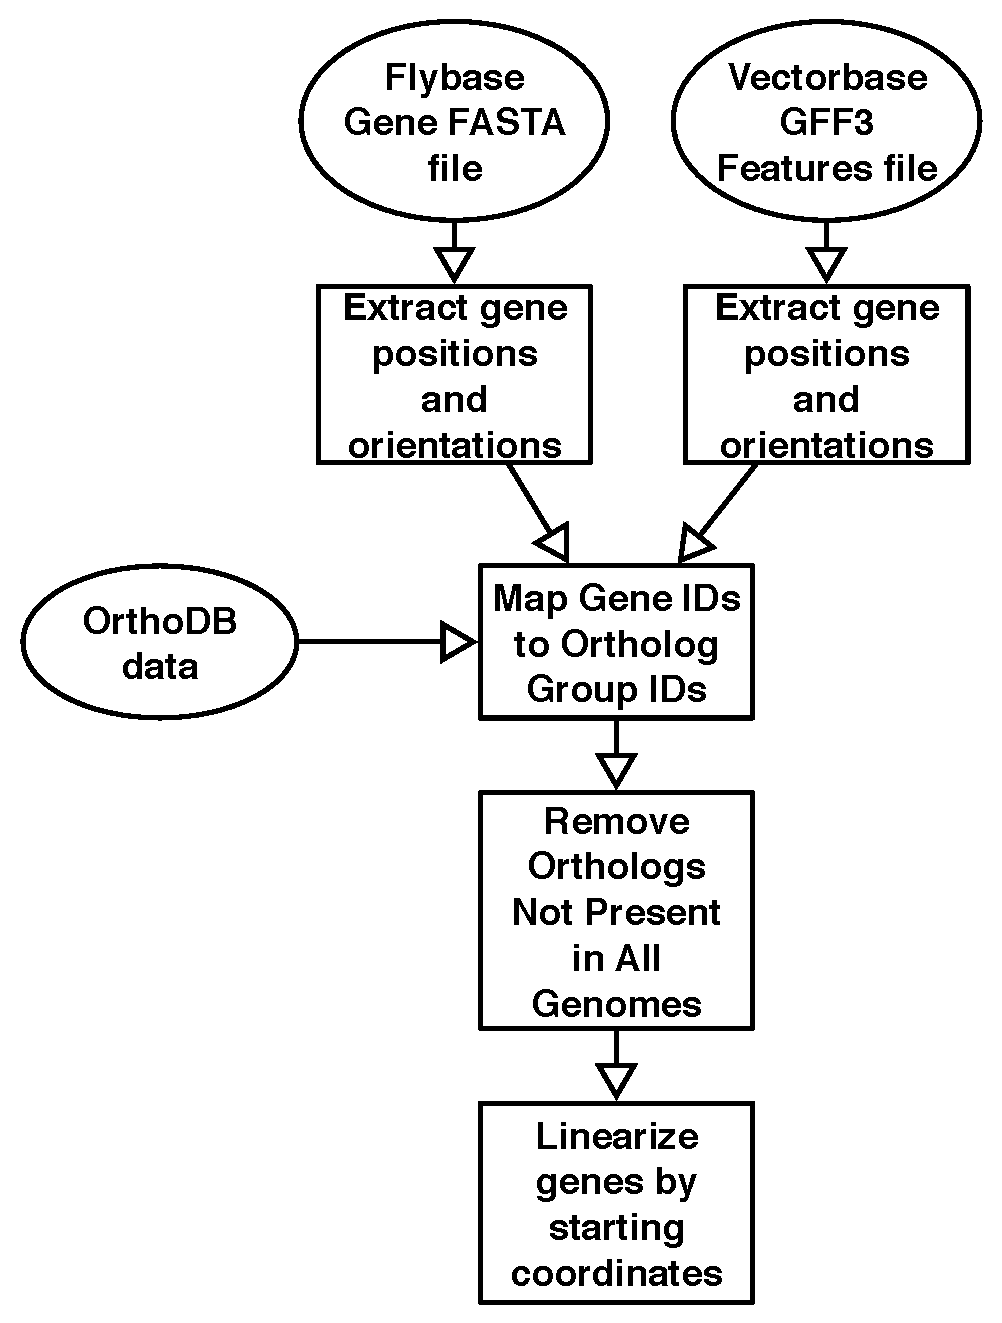
\includegraphics[width=0.5\textwidth]{figures/synteny/orthodb_dotplot_workflow}
  \caption{Workflow for Synteny}
  \label{fig:synteny-workflow}
\end{figure}

\subsubsection{Microsynteny}
For each genome, the identifiers, protein sequences, orientations, scaffolds, and locations extracted from FASTA files for each genome and reformatted as input for the program \texttt{Synchro} \textcolor{red}{TODO CITE}.  \texttt{Synchro} ($\Delta=5$) was run on the pairs \emph{D. melanogaster} and \emph{D. simulans}, \emph{An. gambiae} and \emph{L. longipalpis}, \emph{An. gambiae} and \emph{Ae. aegypti}, and \emph{L. longipalpis} and \emph{P. papatasi}.  Synteny blocks were extracted from the \texttt{OrthBlocks synt} files.  Three-way synteny blocks for \emph{An. gambiae}, \emph{L. longipalpis}, and \emph{P. papatasi} were constructed by finding all pairs of synteny blocks for \emph{An. gambiae} and \emph{L. longipalpis} and \emph{L. longipalpis} and \emph{P. papatasi} that overlapped by at least one gene.  

\textcolor{red}{TODO annotation of synteny blocks, distribution plots}


\subsection{Results}

\subsubsection{Genome Assembly Analysis}

\textcolor{red}{TODO DESCRIPTION}

\begin{figure}[H]
  \centering
  \begin{subfigure}[b]{0.45\textwidth}
    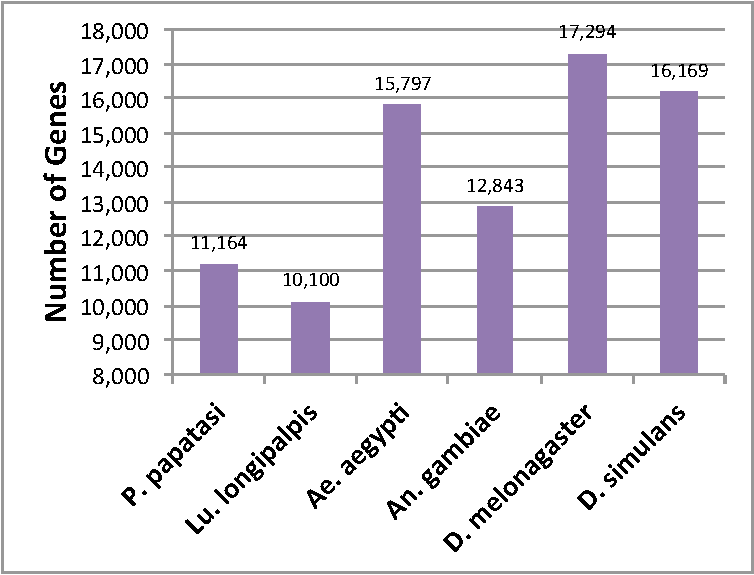
\includegraphics[width=\textwidth]{figures/synteny/genome_size_genes.pdf}
    \caption{Genome Sizes (Genes)}
  \end{subfigure}
  ~
  \begin{subfigure}[b]{0.45\textwidth}
    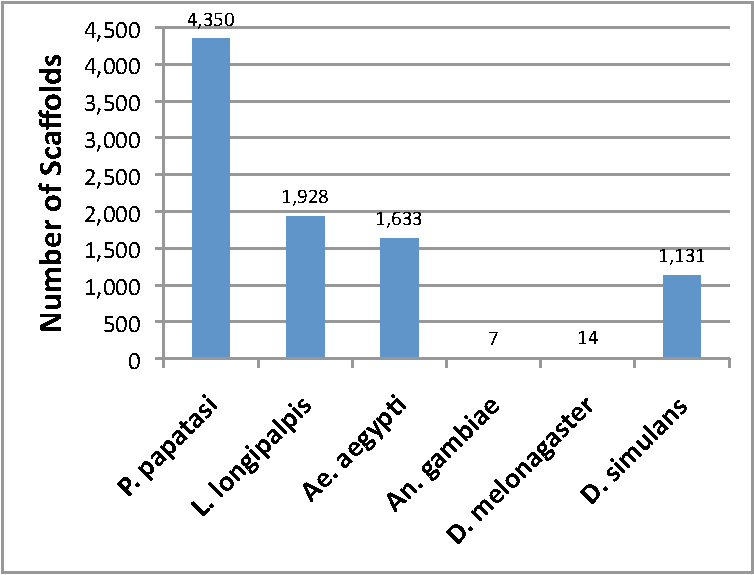
\includegraphics[width=\textwidth]{figures/synteny/scaffold_counts.pdf}
    \caption{Number of Scaffolds}
  \end{subfigure}
  ~
  \begin{subfigure}[b]{0.45\textwidth}
    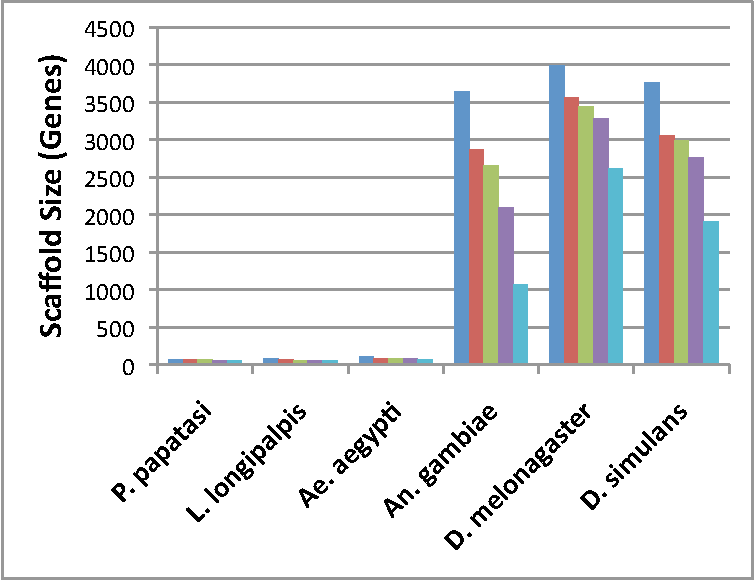
\includegraphics[width=\textwidth]{figures/synteny/top5_scaffold_sizes.pdf}
    \caption{Top 5 Scaffold Sizes (Genes)}
  \end{subfigure}
  ~
  \begin{subfigure}[b]{0.45\textwidth}
    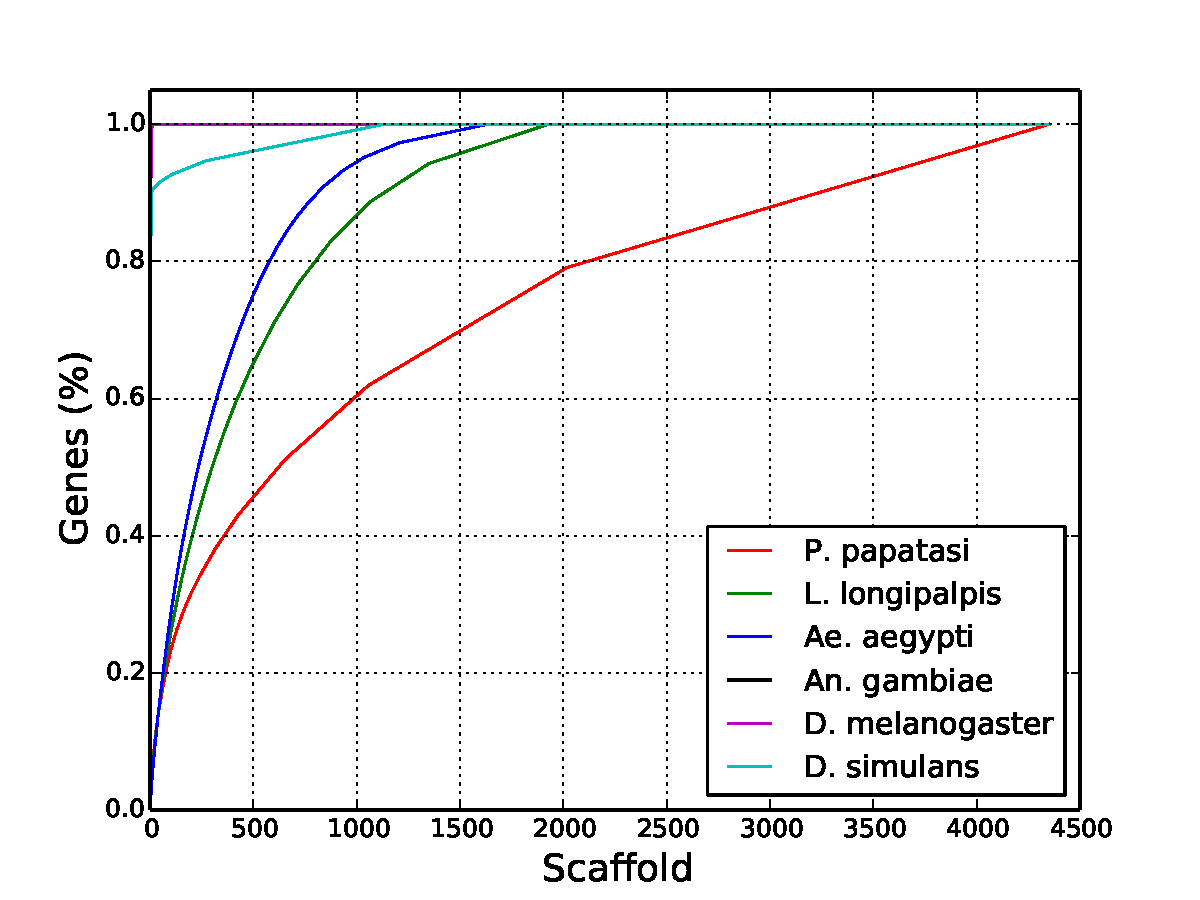
\includegraphics[width=\textwidth]{figures/synteny/gene_scaffold_cdf.pdf}
    \caption{Scaffold Genes CDF}
  \end{subfigure}
  \label{fig:scaffolds}
  \caption{}
\end{figure}

\subsubsection{Analysis of Macrosynteny}
Qualitative comparison of the \emph{L. longipalpis} and \emph{P. papatasi} genomes does not indicate the presence of macrosynteny (Figure~\ref{fig:synteny-dotplots-sandflies}).  Similarly, comparison of the \emph{Ae. aegypti} and \emph{A. gambiae} genomes also fail to demonstrate the presence of synteny (Figure~\ref{fig:synteny-dotplots-mosquitoes}).

In contrast, comparison of the \emph{D. melanogaster} and \emph{D. simulans} genomes indicates extensive presence of synteny (Figure~\ref{fig:synteny-dotplots-drosophila}).  Comparison of the \emph{A. gambiae} and \emph{D. melanogaster} genomes suggest some evidence of synteny but qualitative analysis alone is not sufficient to make a determination (Figure~\ref{fig:synteny-dotplots-anopheles-drosophila}).


\begin{figure}[H]
  \centering
  \begin{subfigure}[b]{0.45\textwidth}
    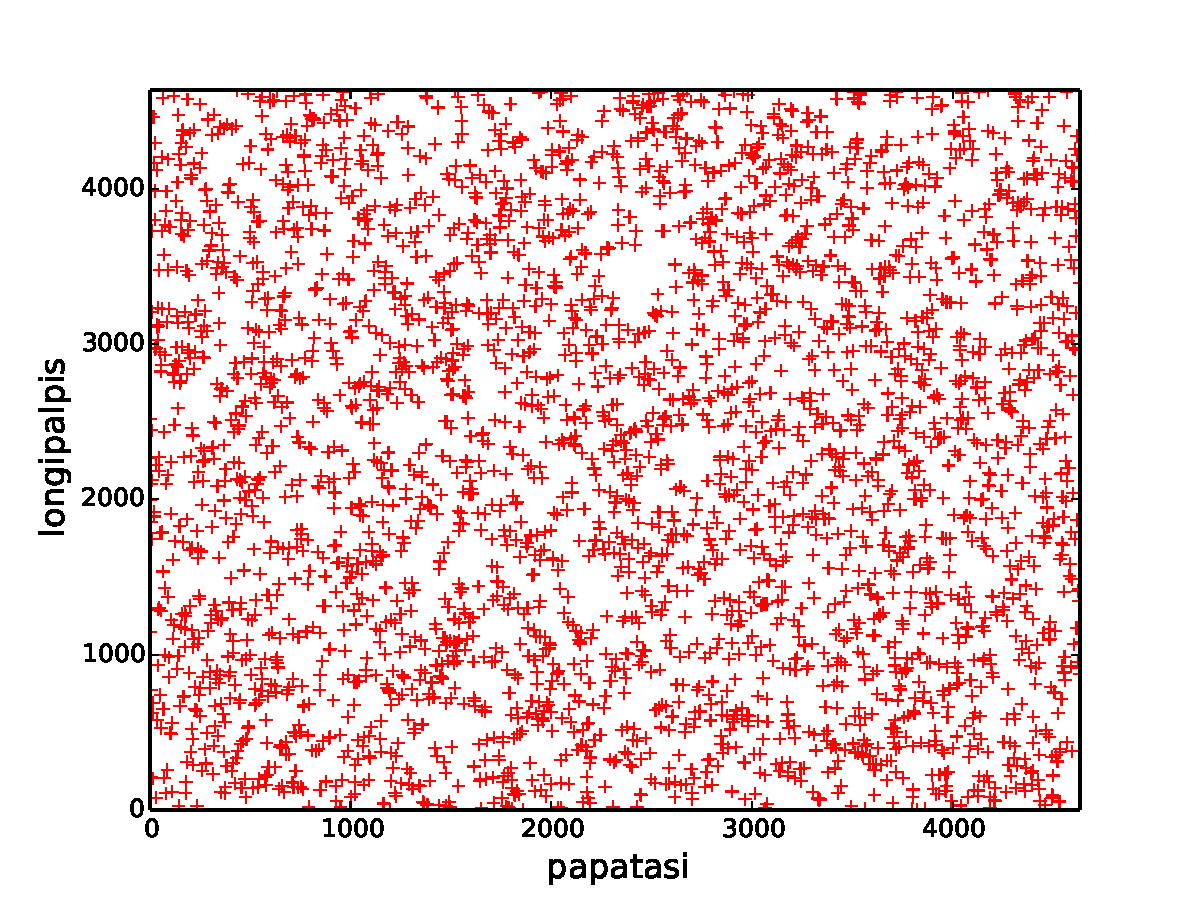
\includegraphics[width=\textwidth]{figures/synteny/papatasi_longipalpis_plot}
    \caption{\emph{L. longipalpis} vs. \emph{P. papatasi}}
    \label{fig:synteny-dotplots-sandflies}
  \end{subfigure}
  ~
  \begin{subfigure}[b]{0.45\textwidth}
    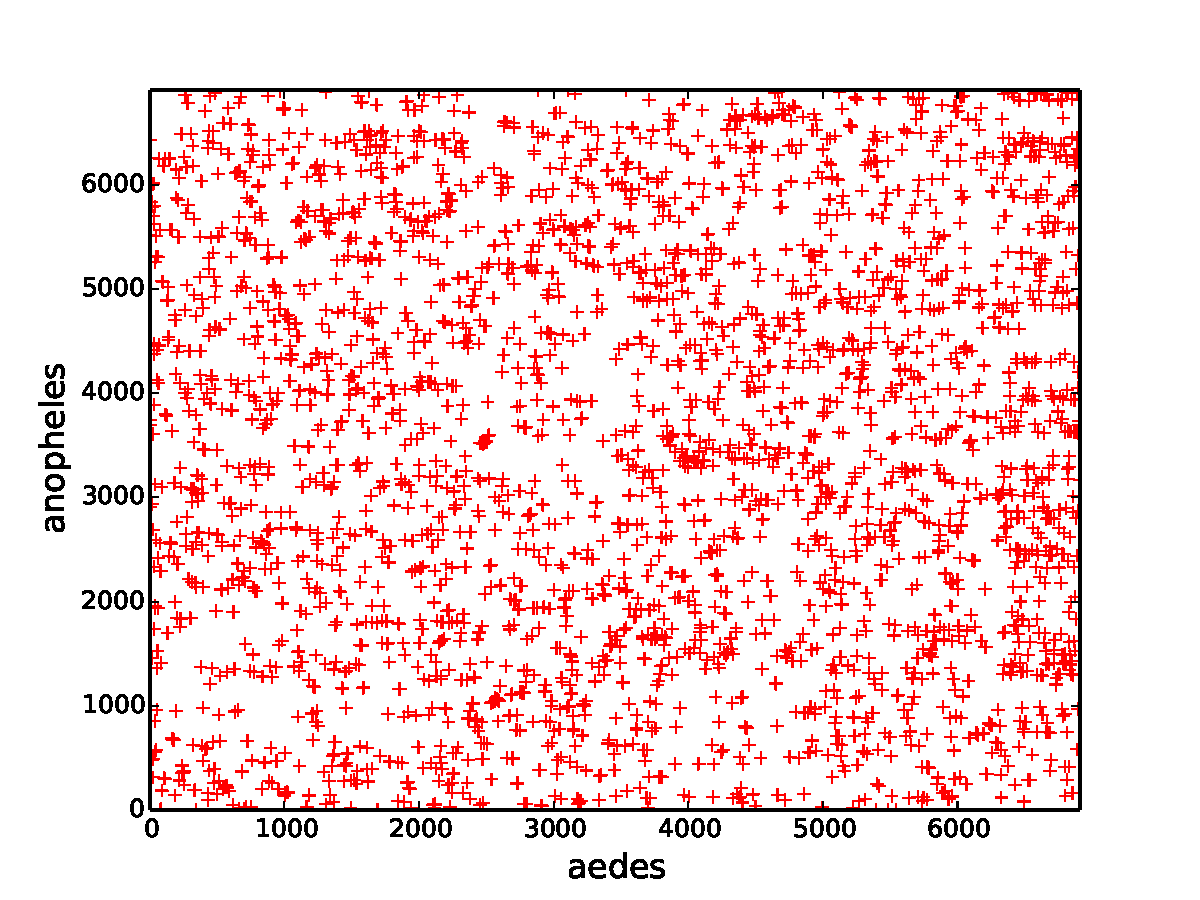
\includegraphics[width=\textwidth]{figures/synteny/aedes_anopheles_plot}
    \caption{\emph{Ae. aegypti} vs. \emph{A. gambiae}}
    \label{fig:synteny-dotplots-mosquitoes}
  \end{subfigure}
  ~
  \begin{subfigure}[b]{0.45\textwidth}
    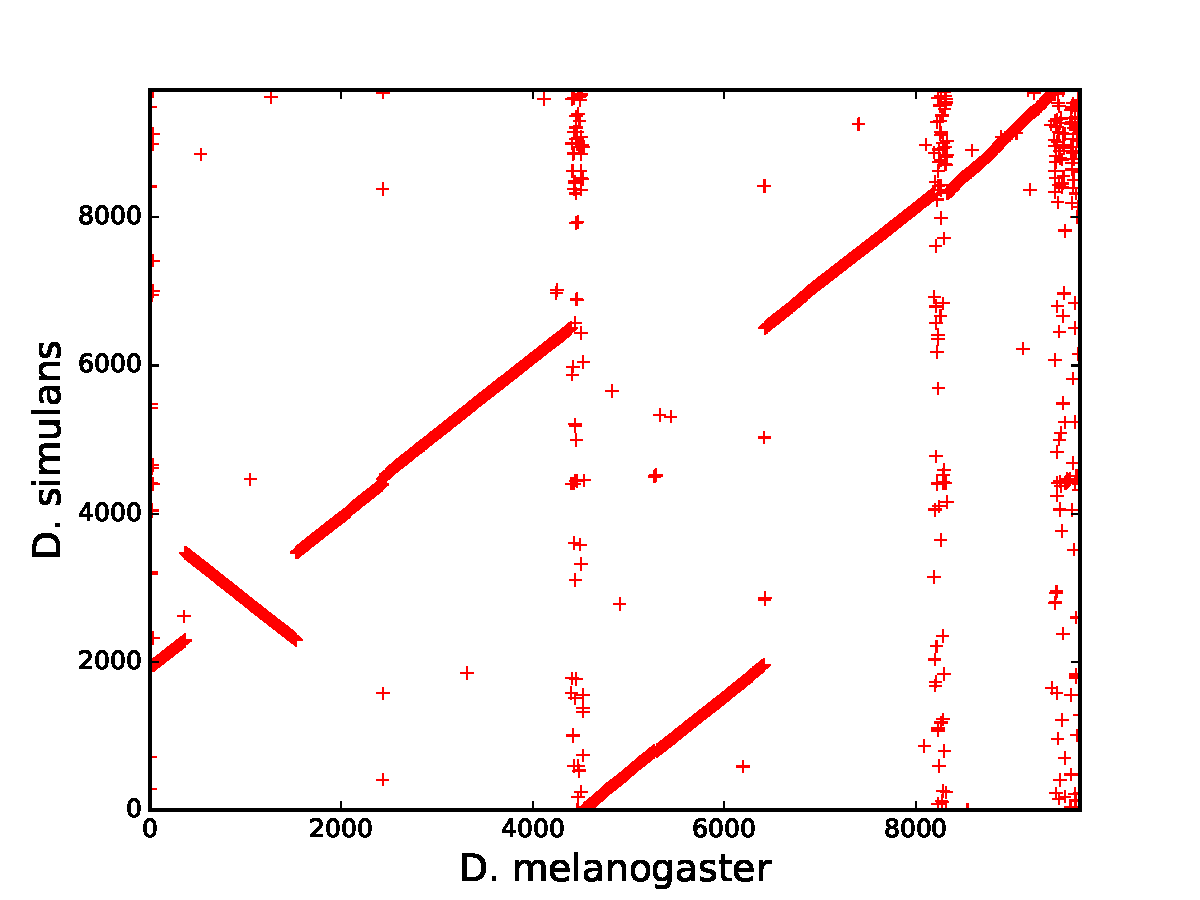
\includegraphics[width=\textwidth]{figures/synteny/dmel_dsim_plot}
    \caption{\emph{D. melanogaster} vs. \emph{D. simulans}}
    \label{fig:synteny-dotplots-drosophila}
  \end{subfigure}
  ~
  \begin{subfigure}[b]{0.45\textwidth}
    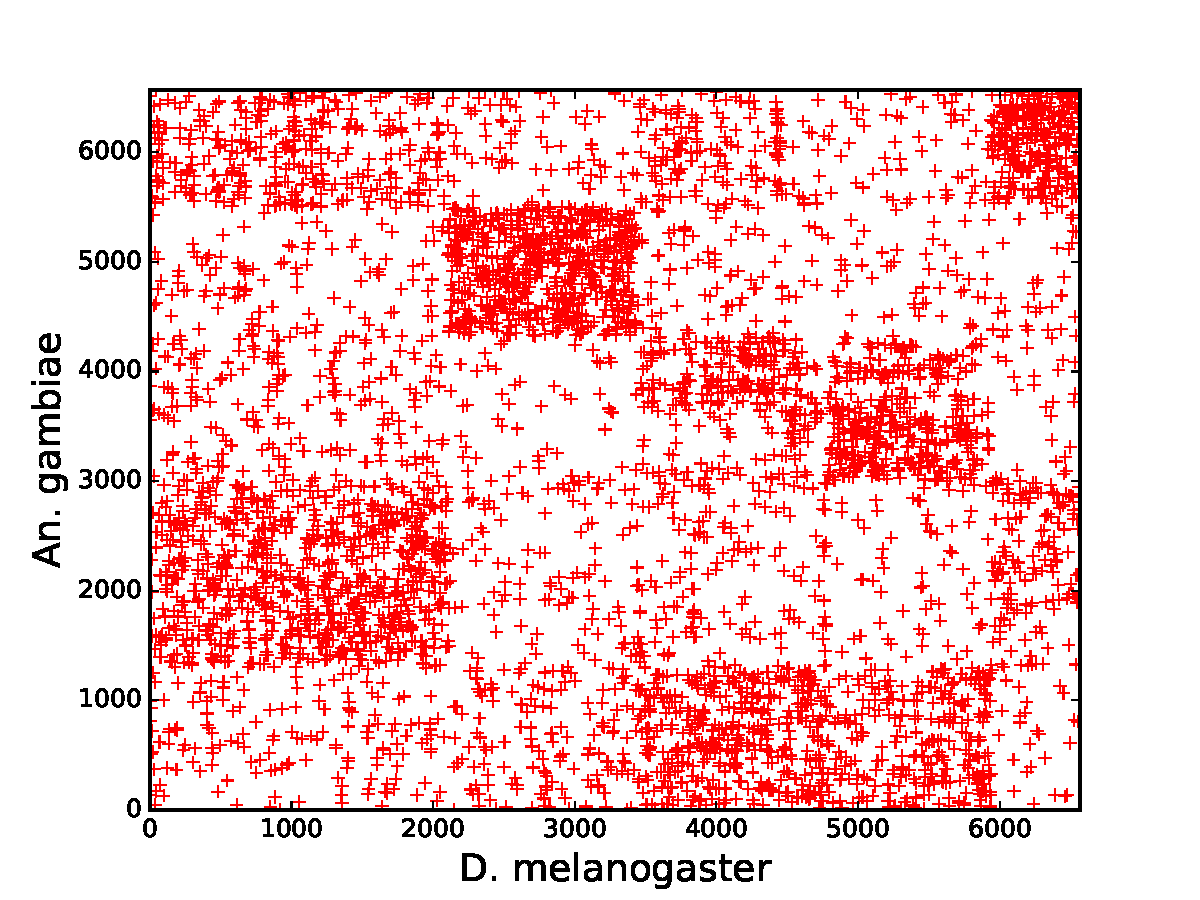
\includegraphics[width=\textwidth]{figures/synteny/dmel_anopheles_plot}
    \caption{\emph{A. gambiae} vs. \emph{D. melanogaster}}
    \label{fig:synteny-dotplots-anopheles-drosophila}
  \end{subfigure}
\label{fig:dot-plots}
\caption{}
\end{figure}

\textcolor{red}{TODO Muller elements}

\subsubsection{Analysis of Microsynteny}

\textcolor{red}{block size distributions}

\textcolor{red}{analysis of individual blocks}

\subsubsection{Annotation of \emph{L. longipalpis} vs. \emph{P. papatasi} Microsynteny Blocks}

\subsection{Discussion and Conclusion}